\documentclass[10pt,a4paper]{article}
\usepackage[latin1]{inputenc}
\usepackage{amsmath}
\usepackage{amsfonts}
\usepackage{amssymb}
\usepackage{graphicx}
\author{Daniel Frederico Lins Leite}
\graphicspath{ {./} }
\newcommand{\qed}{\hfill\blacksquare}
\begin{document}
	
Dasgupta "Algorithms" book:
Exercises:
0.a
\begin{align*}
	f(n) = n - 100\\
	g(x) = n - 200 
\end{align*}
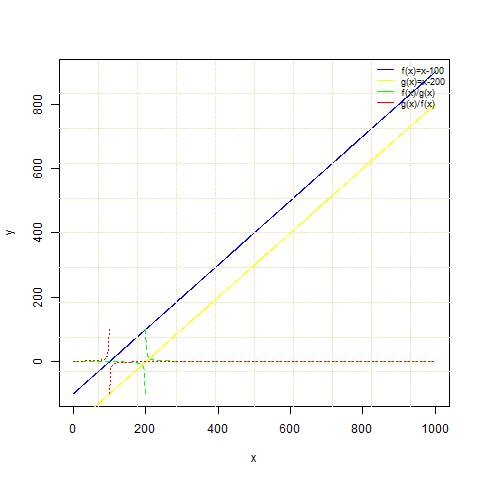
\includegraphics[width=10cm]{0_a.png}
\paragraph{}
Is $f(n)=O(g(n))$?
\begin{align*}
	\frac{n-100}{n-200} = c\\
	n-100=c*(n-200)\\
	n-100=cn-200c\\
	n=cn-200c+100\\
	n-cn=-200c+100\\
	n(1-c)=-200c+100\\
	n=\frac{-200c+100}{1-c}\\
	n=\frac{100(-2c+1)}{1-c}\\
	n=100\frac{-2c+1}{1-c}\\
\end{align*}
\begin{align*}
	n*-1=100\frac{-2c+1}{1-c}*-1\\
	-n=100\frac{2c-1}{-1+c}\\
	-n=100\frac{2c-1}{c-1}\\
	-n=100\frac{2(c-1)}{c-1}\\
	-n=200\frac{c-1}{c-1}\\
	-n=200\\
	n=-200
\end{align*}
\paragraph{}
So
\begin{align*}
	\frac{f(n)}{g(n)}&<=-200*\frac{g(n)}{g(n)}\\
	f(n) &= O(g(n))\\
	\blacksquare
\end{align*}

\paragraph{}
0.2
Show that, if c is a positive real number, then $g(n) = 1 + c + c^2 + ... + c^n$ is:\\
(a) $\theta(1)$ if $c < 1$.\\
(b) $\theta(n)$ if $c = 1$.\\
(c) $\theta(cn)$ if c > 1.\\
The moral: in big-$\theta$ terms, the sum of a geometric series is simply the first term if the series is
strictly decreasing, the last term if the series is strictly increasing, or the number of terms if the
series is unchanging.
\paragraph{}
\begin{align*}
	f(n) &= 1 + c + c^2 + ... + c^n\\
	f(n) &= \sum_{i=0}^{n} {c^i} <= \sum_{i=0}^{\infty} {c^i}\\
	&<=\frac{1}{1-c}
\end{align*}
In the case of $c<1$ we have
\begin{align*}
	f(n) <= \frac{1}{1-c}\\
	f(n) <= z &&z > 0\\
	\frac{f(n)}{g(n)}<=k*\frac{g(n)}{g(n)}\\
	\frac{f(n)}{1}<=k*\frac{1}{1}&&\text{choose $k=z$}\\\\
	f(n) = O(1)\\
\end{align*}
In the case of $c=1$ we have
\begin{align*}
	f(n) &= 1 + 1^2 + ... + 1^n\\
	f(n) &= \sum_{i=0}^{n}{1} = n\\
	\frac{f(n)}{g(n)}&<=k*\frac{g(n)}{g(n)}\\
	\frac{n}{n}&<=k*\frac{n}{n}&&\text{choose $k=1$}\\
	f(n) &= O(n)
\end{align*}
In the case of $c>1$ we have
\begin{align*}
	f(n) &= 1 + c^2 + ... + c^n\\
	f(n) &= \sum_{i=0}^{n} {c^i} <= \sum_{i=0}^{\infty} {c^i}\\
	&=\sum_{i=0}^{\infty} {c^n}\\
	&=c^n*\sum_{i=0}^{\infty} {1}\\
	&=n*c^n\\
	f(n)&<=n*c^n\\
	\frac{f(n)}{g(n)}&<=k*\frac{g(n)}{g(n)}\\
	\frac{f(n)}{c^n}&<=k*\frac{c^n}{c^n} &&\text{choose $k=n$}\\
	f(n) &= O(c^n)
	\blacksquare
\end{align*}

0.3
The Fibonacci numbers F 0 ,F 1 ,F 2 ,..., are defined by the rule
F 0 = 0, F 1 = 1, F n = F n?1 + F n?2 .
In this problem we will confirm that this sequence grows exponentially fast and obtain some
bounds on its growth.
(a) Use induction to prove that F n ? 2 0.5n for n ? 6.
(b) Find a constant c < 1 such that F n ? 2 cn for all n ? 0. Show that your answer is correct.
(c) What is the largest c you can find for which F n = ?(2 cn )?

(a)
missing bases steps
\begin{align*}
F_n &>= 2^{n/2}\\
F_n &= F_{n-1}+F_{n-2}\\
&>= 2^{(n-1)/2} + 2^{(n-2)/2}\\
& &= (X+2^{(n-2)/2}) + 2^{(n-2)/2} &&\text{$X>0$}\\
& &= 2*2^{(n-2)/2}\\
&>= 2*2^{(n-2)/2}\\
& &=2^{\frac{n-2}{2}+1}\\
& &=2^{\frac{n-2}{2}+\frac{2}{2}}\\
& &=2^{\frac{n}{2}}\\
&>= 2^{n/2}\\
\qed
\end{align*}

(B)
\begin{align*}
	F_n &<= 2^{cn}\\
	F_{n-2} + F_{n-1} &<= 2^{cn}\\
	2^{c(n-2)} + 2^{c(n-1)} &<= 2^{cn}\\
	2^{cn-2c} + 2^{cn-c} &<= 2^{cn}\\
	\frac{2^{cn}}{2^{2c}} + \frac{2^{cn}}{2^c} &<= 2^{cn}\\
	\frac{(2^{c})^n}{(2^{c})^2} + \frac{(2^{c})^n}{2^c} &<= (2^{c})^n\\
	\frac{a^n}{a^2} + \frac{a^n}{a} &<= a^n\\
	\frac{aa^n}{aa^2} + \frac{a^2a^n}{a^2a} &<= a^n\\
	\frac{a^{n+1}}{a^3} + \frac{a^{n+2}}{a^3} &<= a^n\\
	\frac{a^{n+1}}{a^3} + \frac{a^{n+2}}{a^3} &<= a^n\\
	\frac{a^{n+1}+a^{n+2}}{a^n} &<= a^3\\
	\frac{aa^n+a^2a^n}{a^n} &<= a^3\\
	\frac{a^n(a+a^2)}{a^n} &<= a^3\\
	a+a^2 &<= a^3\\
	2^c+2^{2c}&<=2^{3c}\\
	\log_2{(2^c+2^{2c})}&<=\log_2{(2^{3c})}\\
\end{align*}
Fib
0
1
1
2
3
5
8
13
21
34
55
89
144
233
377
610
987
1597
2584
4181
6765
\end{document}